\documentclass[10pt]{article}

\usepackage{../Utils}
\usepackage{eurosym}
\bc
Internet connections no longer slow and haperend. e-mail clients now have ajax interfaces. More small terminals (phones etc.) Time is ripe to make server based editors. Allowing advanced editing on these machines.


VNC shows that it works. Latency is a problem. will get better, and also Proxima can do much better than that.



Ajax front end for Proxima


Proxima's layered architecture makes it relatively easy to change the front end. In fact, a previous version made use of a stand-alone renderer that communicated through a socket. Incrementality takes care that minimal updates are sent to the renderer.

Two components change: the renderer and the GUI module that is the current event loop.

The renderer will be modified to produce XML strings instead of rendering commands. 

The GUI event loop will become a HTTP server that takes requests (edit gestures) lets Proxima handle these and sends the resulting XML from the rendering back to the client.

Apart from this, we need an Ajax front-end in Java script. It should render the XML commands received from Proxima, and capture user edit gestures.


Links:

graphical elements:
http://www.walterzorn.com/jsgraphics/jsgraphics_e.htm

key events:
http://unixpapa.com/js/key.html

mouse events:
http://javascript.internet.com/page-details/mouse-coordinates.html
http://unixpapa.com/js/testmouse.html

Open questions:

Where is the source located? What happens to images? Efficiency of client when many strings are present?

Need to encode rendering? 
\ec



\bc

    * Introduction --short description of the project and goals;
    * Description of innovation:
          o the problem solved by this project;
          o the relative advantage of the proposed innovation;
          o usability: for whom and to what purpose;
          o perspectives for further development of this innovation and/or other technologies. 
    * Project setup --organizational, technical, eventual partners, dependencies on other projects, licenses, and such;
    * Project planning --milestones and related results;
    * Project budgeting;
    * Project risks --which risks can be overseen from the start of the project;
    * Project results dissemination --how the project team is going to disseminate results and to whom, publicity, diffusion of the produced innovation;
    * Possibly, follow-ups on the project. 

\ec



\title{Web-based generic editing}
\author{dr. Martijn M. Schrage}
\date{\version}
\begin{document}
\maketitle

\section{Introduction}
%    * Introduction --short description of the project and goals;

Web 2.0 is advancing. users edit pages. Text only. Wikipedia (more examples) Formula is plain text. Wysiwyg editing is interesting. Ajax, DHTML and Flash make it possible to create them (eg. Yahoo pipes), but difficult to build them.

Moreover, editors put a burden on the client. Clients are getting smaller, and internet is getting more stable. So it makes sense to take the editing away from the local device and make a server based editor. VNC shows this to be possible.

vb google docs


The Proxima generic editor can offer wysiwyg editors that can be constructed with little effort. Specifying a document type, a presentation and the edit behavior, a editor is created quickly.

Because of its architecture, it is rather straightforward to provide Proxima with a web-interface. Instead of rendering the presentation on a screen, it is an HTTP server that sends the rendering and updates to a client. The client has a lightweight Ajax renderer that draws the screen and captures mouse and keyboard events.

The web-based Proxima can provide wysiwyg editors. That expect very little from a client. Moreover, graphical editors can be built easily. 



\section{Project description}
%    * Description of innovation:
%          o the problem solved by this project;
%          o the relative advantage of the proposed innovation;
%          o usability: for whom and to what purpose;

\subsection{The problem(?)} 

Web-based editing. Either built in text fields, such as most wikis. Or custom made editors written in Flash or Javascrips. Yahoo pipes, Google docs.

Internet getting faster. Devices getting smaller. 

\subsection{Proxima}
Proxima. What is proxima and generic editing

Proxima is an generic editor is system that can be used to create editors. Can be easily extended to run server-based with a light client.

Editor for documenting Bayesian networks. Network and views on this network. check consitencies.

\begin{figure}
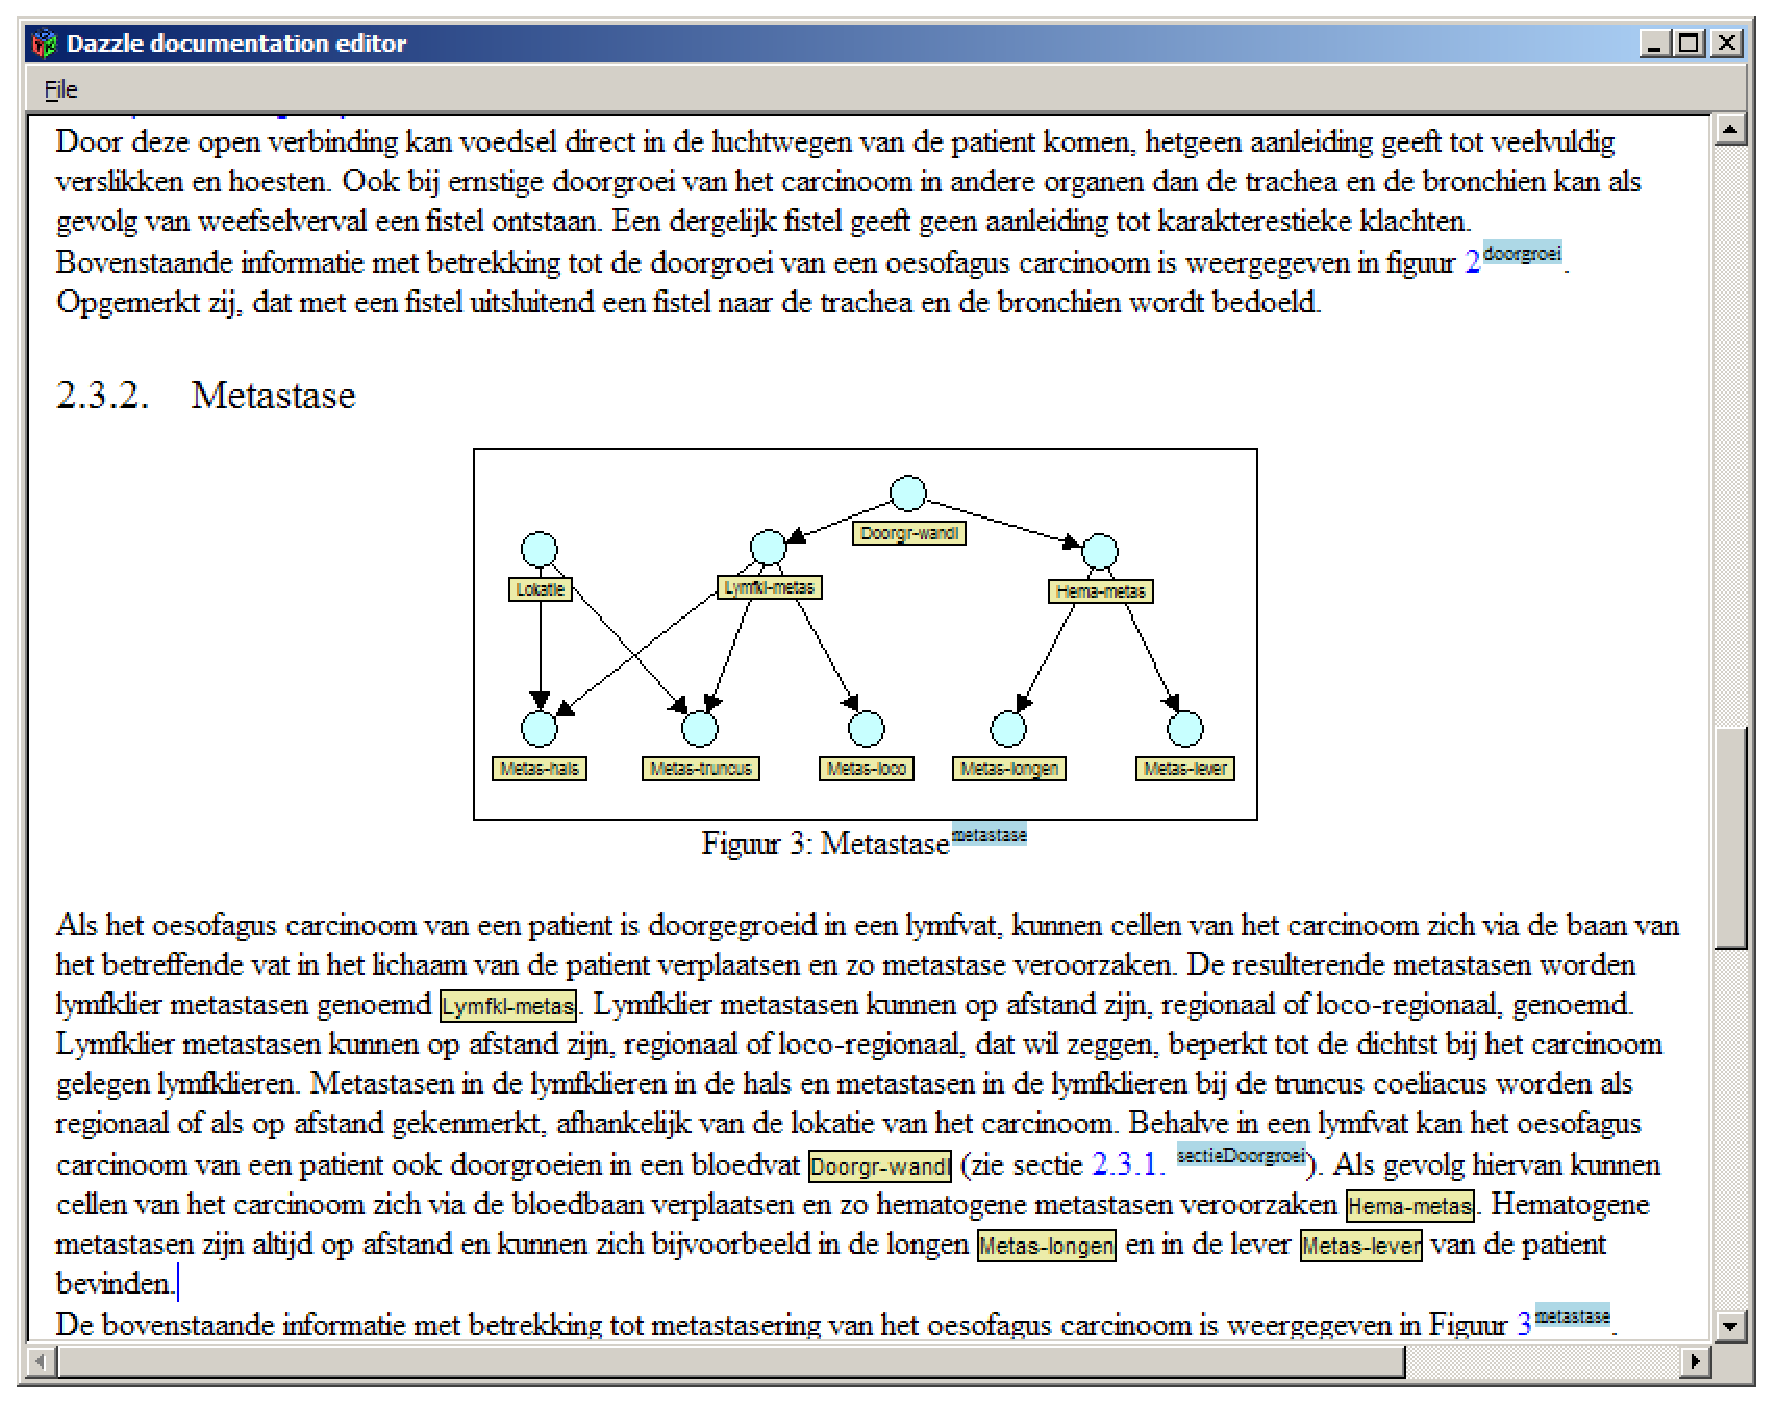
\includegraphics[width=12cm]{images/subgraph}
\caption{The Bayesian network documentation editor.}
\label{fig:levelsAndLayers}
\end{figure}

Another bla.

General description of what Proxima is good for.


\subsection{The Proxima architecture}

The core architecture of Proxima consists of a number of layers, each communicating with its direct neighbors. The layered structure is based on the staged nature of the {\em presentation} process and its inverse, the {\em interpretation} process. The positions at which the document, the rendering, and the intermediate data structures reside are called {\em levels}. Between each pair of levels we have a {\em layer} that maintains the mappings between its adjacent levels. Each layer consists of a presentation component and an interpretation component and may be parameterized by a {\em sheet}. Figure~\ref{fig:levelsAndLayers} schematically shows the levels and layers of Proxima. From a document type definition, a code generator generates a number of Haskell modules, which are compiled together with the sheets and the Proxima base modules to yield an editor. 

\begin{figure}
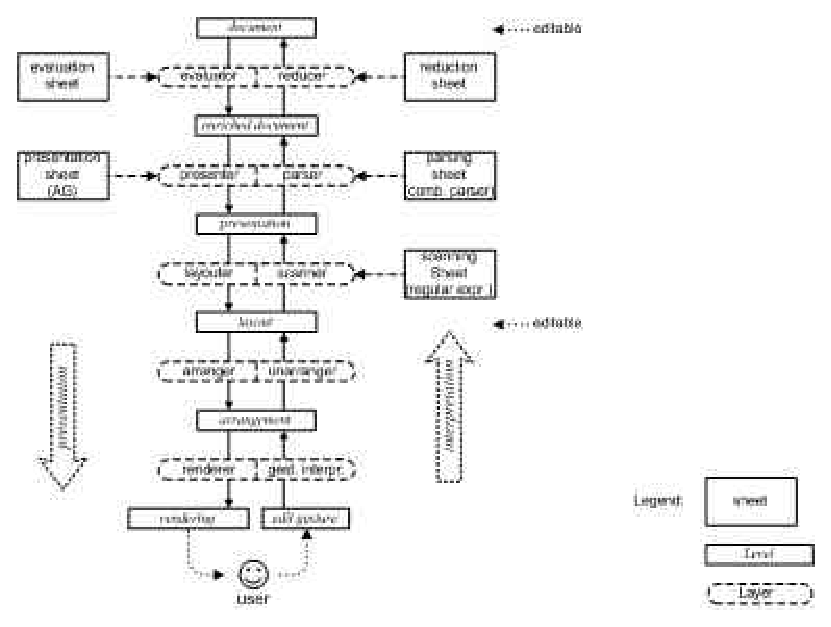
\includegraphics[width=12cm]{images/LayerOverview}
\caption{The levels and Layers of Proxima.}
\label{fig:levelsAndLayers}
\end{figure}

A data level in Proxima is not simply an intermediate value in the presentation computation. It is an entity in its own right and maintains part of the state of the editor. The six levels of Proxima are:


\bl
\o {\bf Document:} The document structure.

\o {\bf Enriched Document:} The document attributed with derived values and structures, such as the type of a function or a table of contents, typically computed by an attribute grammar~\cite{reps84synGen}.

\o{\bf Presentation:} A logical description of the presentation of the document, consisting of rows and columns of presentation elements with attributes. The presentation also supports formatting based on available space (e.g.\ line breaking).

\o{\bf Layout:} A presentation with explicit white space, which does not contain tokens.

\o{\bf Arrangement:} A formatted layout with absolute size and position information.

\o{\bf Rendering:} A bitmap of the arrangement.
\el


Discuss sheets.

\bc
We briefly discuss each of the five layers.

\head{Evaluation layer}\\
The evaluation layer takes care of computing derived structures and values over the document, and of mapping updates on these derived structures back to document updates. In this layer, for example, type inference may take place. The layer is parameterized by an {\em evaluation sheet} and a {\em reduction sheet}, which specify the mappings. 

\head{Presentation layer}\\
The presentation layer consists of the presenter and the parser. The presenter takes an enriched document tree and computes a presentation for it according to the {\em presentation sheet}. Its counterpart, the parser, maps a presentation tree back to an enriched document and is parameterized by a {\em parsing sheet}.

\head{Layout layer}\\
The layout layer handles automatic white space, which is maintained in the white-space map that is part of the presentation level. For each token, the layout component looks up the corresponding white space and inserts actual line breaks and spaces in the presentation. The scanner recognizes tokens in the layout level, based on regular expressions specified in the {\em scanning sheet}. It also stores white space in the white-space map. Because mapping tokens to strings is straightforward, the layout component does not need a sheet parameter.

\head{Arrangement layer}\\
In the presentation direction, the arrangement layer computes the precise position and size for each element in the layout level. It also handles line breaking. The arrangement level is not directly editable, so it need not be mapped back onto the layout level. Hence, the only thing that needs to be done in the interpretation direction, is to map absolute coordinates in edit commands to paths in the presentation tree. 

\head{Rendering layer}\\
The renderer creates a bitmap for the arrangement. In the other direction is the gesture interpreter, which maps edit gestures onto edit operations designated for the higher layers.

\ec

%\bl
%\o implementation: layer combinators.
%\o sometimes awkward, because we have to conform to the layers.
%\o but this has advantages: new GUI lib in a matter of days.
%\el




Presentation-oriented editing actually takes place at the layout level rather than the presentation level, thus allowing free-text editing also on white space (which is absent on the presentation level). Hence the two levels that are directly editable are the document level and the layout level. After an edit operation on the document, all levels from document to rendering are updated to reflect the update. After an edit operation on the layout level, the modified layout is scanned, parsed and reduced, to obtain the corresponding updated document, from which an updated rendering is computed. Scanning and parsing does not occur after every presentation edit operation. Depending on the editor, it may occur either on a navigation operation, after a certain time interval, or at an explicit request by the user.


\subsection{A web-based Proxima}

A web-based Proxima requires the development of three aspects:
\bl
\o An Ajax client that renders a presentation (or part of it) on the screen and captures key and mouse events, sent back as edit commands to the server.
\o An HTTP server that sends a rendering to a client and retrieves the edit commands.
\o A Proxima rendering module that renders to a string based format that is handled by the client.
\el

Proxima is layered. Separation. Gui specific stuff only in a couple of places. Changing to different GUI library is a matter of days. In fact the early version had a stand-alone renderer that was being communicated with through a socket.

\subsubsection{HTTP server}

Currently the GUI module. Event loop that catches an event. Creates an edit command that is sent to Proxima. The result is a rendering (now a set of gui commands) which is drawn on a buffer.

Rather than a GUI event loop. It becomes an HTTP server. Incoming connections
 
\subsubsection{The web-based renderer}
The current renderer creates gui commands for GTK. It walks over arrangement data structure that describes the positions. For changed parts, commands are generated. New renderer rather similar, but will generate a string. 

\subsubsection{Ajax client}

Main project. Use DHTML to update rendering.

Because of latency, edit operations must be collected. Because focus is known, typed characters can be added to the string containing the focus.

\subsection{Further development}
%          o perspectives for further development of this innovation and/or other technologies. 
Works well enough for small docs. 


\section{Project planning}
%    * Project setup --organizational, technical, eventual partners, dependencies on other projects, licenses, and such;



%    * Project planning --milestones and related results;
investigate Ajax an DHTML technologies
setup implement Ajax client
determine format of rendering

first just socket thing
sending simple tree rep.
later full http. with the url describing the document to be edited.
later better string encoding

%    * Project budgeting;

30.000 \euro

%    * Project risks --which risks can be overseen from the start of the project;

%    * Project results dissemination --how the project team is going to disseminate results and to whom, publicity, diffusion of the produced innovation;

Tja..

%    * Possibly, follow-ups on the project. 

With more incremental behavior, larger editors can be written. Application for NWO is on its way.



\bibliographystyle{plain}
\bibliography{../proxima}

\end{document}